\subsection{Giới thiệu}
Sau khi hoàn thành quá trình huấn luyện mô hình nhận diện ngôn ngữ độc hại, bước tiếp theo là áp dụng mô hình này vào thực tiễn để giải quyết các vấn đề thực tế. Trong phần này, chúng tôi sẽ trình bày hai ứng dụng cụ thể của mô hình: một tiện ích sử dụng trên Chrome và một chatbot Discord.

Hai ứng dụng này không chỉ minh họa cho khả năng ứng dụng của mô hình nhận diện ngôn ngữ độc hại mà còn mở ra nhiều cơ hội mới cho việc bảo vệ người dùng trước các nguy cơ từ ngôn ngữ tiêu cực trên Internet.

\subsection{Mục đích}

Tiện ích Chrome được thiết kế nhằm giúp người dùng trình duyệt web có thể nhận diện và cảnh báo về các nội dung độc hại trực tiếp trên các trang web mà họ truy cập. Với việc tích hợp mô hình học máy đã được huấn luyện, tiện ích này có thể phân tích và đánh giá nội dung trang web trong thời gian thực, từ đó cảnh báo người dùng khi phát hiện các ngôn ngữ độc hại.

Ứng dụng thứ hai của mô hình là một loại chatbot được tích hợp vào nền tảng Discord. Discord là một ứng dụng chat phổ biến, đặc biệt trong cộng đồng game thủ và các nhóm học tập, làm việc. Việc sử dụng chatbot có khả năng nhận diện ngôn ngữ độc hại sẽ giúp duy trì một môi trường giao tiếp an toàn và lành mạnh. Chatbot này có khả năng giám sát các cuộc trò chuyện trong thời gian thực, phát hiện và phản hồi ngay lập tức khi phát hiện ngôn ngữ độc hại.

\subsection{Quá trình phát triển}
Để triển khai mô hình nhận diện ngôn ngữ độc hại vào thực tiễn dưới dạng tiện ích Chrome và chatbot Discord, chúng tôi đã xây dựng một API Server sử dụng framework Flask của Python. API Server này được triển khai trên nền tảng Hugging Face, giúp tạo ra một hệ thống đơn giản, hiệu quả và tiết kiệm chi phí.

Cả hai ứng dụng sẽ gửi các nội dung cần phân tích đến API Server, sau đó nhận kết quả từ mô hình nhận diện ngôn ngữ độc hại. Dựa vào kết quả này, tiện ích Chrome sẽ đánh dấu các nội dung độc hại trên trang web, còn chatbot Discord sẽ phản hồi ngay lập tức khi phát hiện ngôn ngữ độc hại trong cuộc trò chuyện.

\subsection{Cách hoạt động}

\subsubsection{Tiện ích Chrome}
\begin{figure}[htb!]
    \begin{subfigure}[b]{0.33\textwidth}
        \centering
        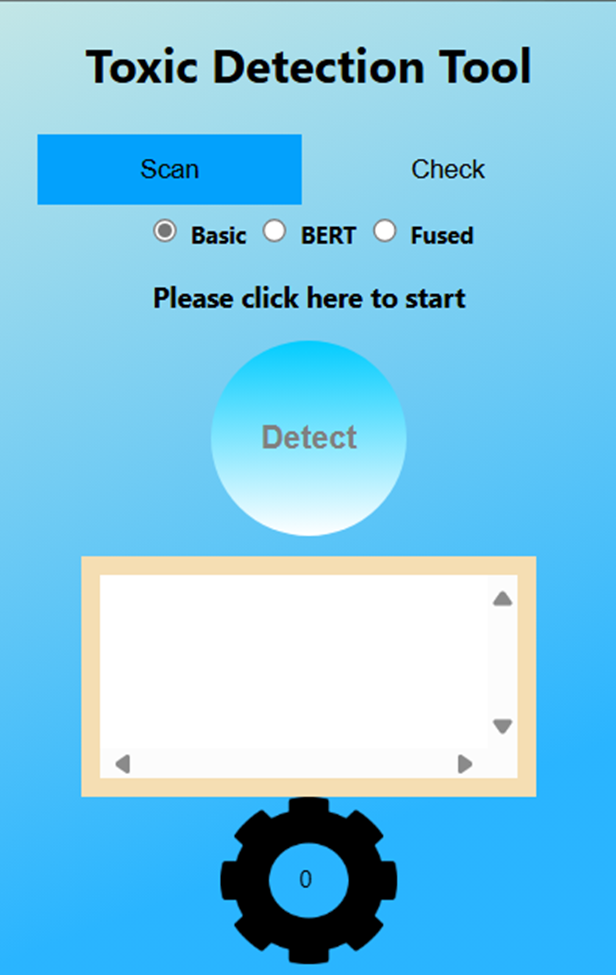
\includegraphics[width=0.8\textwidth]{image/ex_web.png}
        \caption{Tiện ích: Quét nội dung toàn bộ trang web}
        \label{figure:ex_web}
    \end{subfigure}%
    \begin{subfigure}[b]{0.33\textwidth}
        \centering
        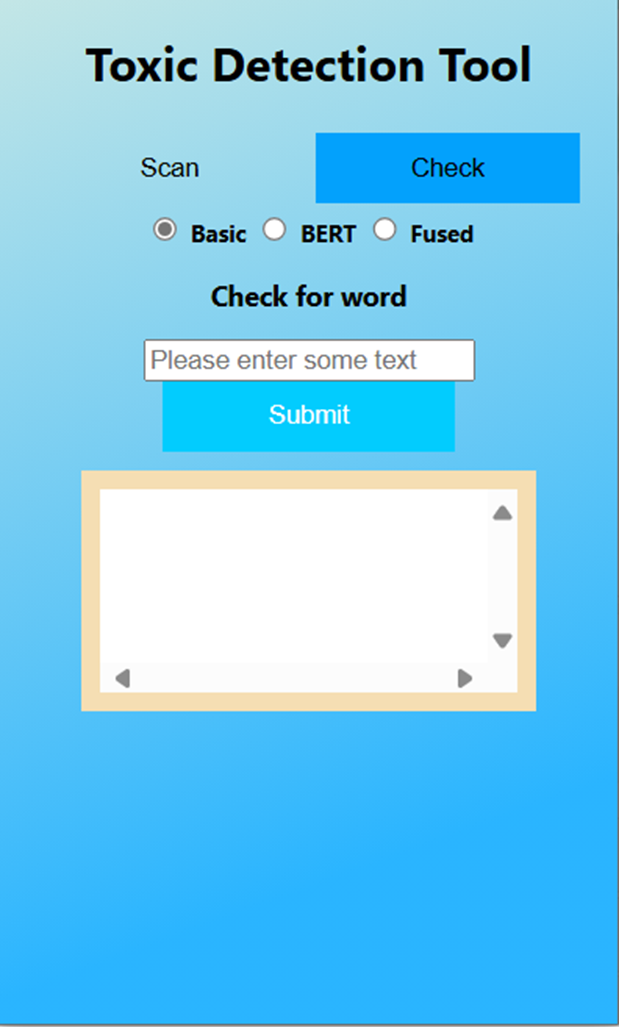
\includegraphics[width=0.8\textwidth]{image/ex_text_enter.png}
        \caption{Tiện ích: Nhập văn bản cần xác định độ độc hại}
        \label{figure:ex_text_enter}
    \end{subfigure}%
    \begin{subfigure}[b]{0.33\textwidth}
        \centering
        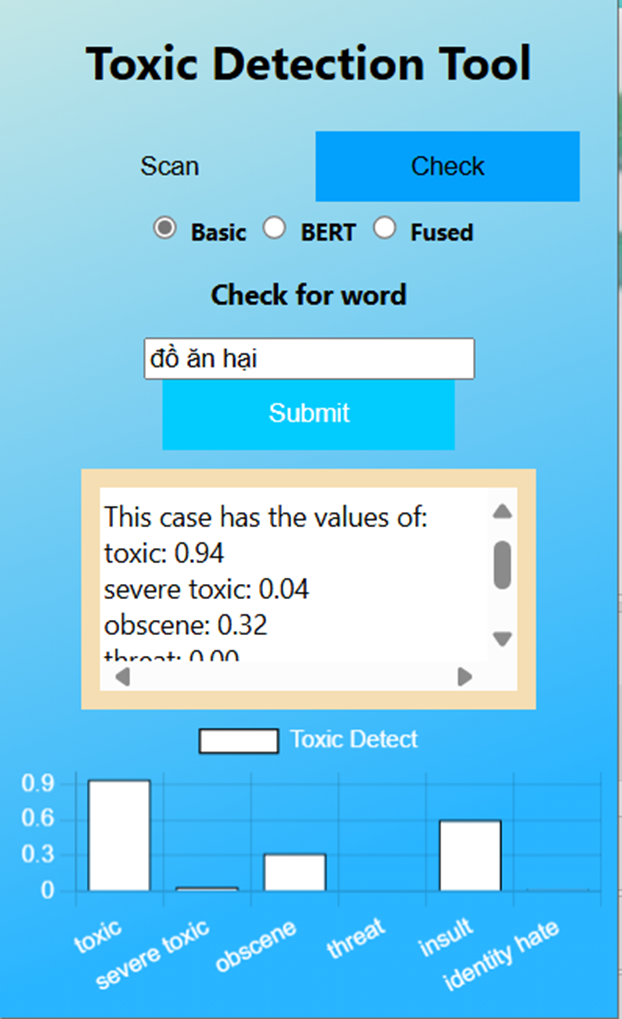
\includegraphics[width=0.8\textwidth]{image/ex_text_eval.png}
        \caption{Tiện ích: Đánh giá mức độ độc hại của văn bản}
        \label{figure:ex_text_eval}
    \end{subfigure}
    \caption{Tổng quan tiện ích Chrome}
\end{figure}

Tiện ích Chrome sẽ quét lấy các nội dung dạng chữ trên trang web và gửi về cho API Server, dựa vào kết quả sẽ biết được các bình luận độc hại hay không. Có 2 mức độc hại là độc hại và rất độc hại. Sau khi có kết quả, người dùng có thể chọn làm nổi bật hoặc ẩn đi các bình luận tiêu cực. Với các nội dung ở mức độc hại, các nội dung này sẽ được làm nổi lên bằng cách tô đỏ. Với các nội dung ở mức rất độc hại, các nội dung này sẽ được ẩn đi để người dùng không thể nhìn thấy.

Hướng dẫn: Ấn nút Detect để thực hiện quét nội dung. Sau khi có thông báo hoàn thành, các nội dung độc hại sẽ hiển thị ở ô văn bản bên dưới và số lượng bình luận độc hại sẽ hiển thị trong bánh răng phía dưới. Người dùng có thể lọc các bình luận độc hại bằng cách nhấn vào bánh răng.

Ngoài ra, còn có thể kiểm tra độ độc hại của văn bản do người dùng nhập và hiển thị biểu đồ thể hiện mức nghiêm trọng của nội dung đó.

Hướng dẫn: Nhập văn bản cần đánh giá vào ô phía trên và ấn Submit, đánh giá về nội dung đó sẽ được hiển thị ở ô văn bản phía dưới và biểu đồ sẽ hiện ra ở dưới ô kết quả.

\subsubsection{Discord chatbot}
\begin{figure}[htb]
    \centering
    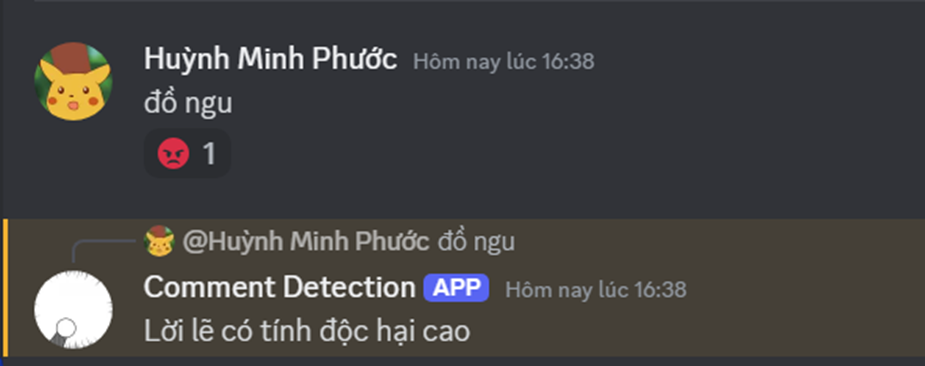
\includegraphics[width=0.5\textwidth]{image/bot_discord.png}
    \caption{Tiện ích: chatbot trên Discord}
    \label{figure:bot_discord}
\end{figure}

Discord chatbot sẽ hoạt động trong các nhóm chat và đánh dấu các nội dung độc hại kèm bình luận và cảm xúc.